\section{Projektidee} % (fold)
\label{sec:projektidee}

\subsection{Bisherige Tower Defense Spiele} % (fold)
\label{sub:bisherige_tower_defense_spiele}
Das Tower Defense Genre (Abk. \emph{TD}) bietet eine große Bandbreite an verschiedenen Umsetzungen. Das Grundkonzept ist dabei immer, dass der Spieler mehrere Wellen an KI-Gegnern, sogenannte \enquote{Creeps}, auf einer Karte davon abhalten muss, bestimmte Ziele zu erreichen. Dazu kann er Türme platzieren, die die Creeps töten. In den meisten Fällen handelt es sich um eher kleinere Spiele, wie Browser-, Flash- oder Mobile Games. Auch die ersten bekannteren TD-Spiele sind als Custom Maps im Warcraft oder StarCraft MapEditor entstanden und haben daher kein großes Entwicklerteam im Hintergrund. Der Umfang war damit für das eigene Projekt gut abschätzbar und der vorgesehenen Bearbeitungszeit angemessen. Vereinzelt wurde das Spielprinzip aber auch in größeren Produktionen, wie Sanctum, aufgegriffen, was die Erweiterbarkeit des Ansatzes zeigt. Es existieren bereits einige Spielvariationen, über die im Folgenden exemplarisch ein Überblick gegeben werden soll.

\paragraph{Klassisches Spiel}
In der häufigsten (da einfachsten) Spielimplementierung bewegen sich die Creeps auf einem vordefinierten Pfad und die Türme werden entlang des Pfades frei oder auf bestimmten Knotenpunkten positioniert. Typischer Weise gibt es unterschiedliche Türme und verschiedene Creep-Arten. Zum Teil haben diese auch Spezialfähigkeiten, wie fliegende Creeps (folgen also nicht dem Pfad, sondern bewegen sich auf direkter Linie zum Ziel) bzw. Türme, die besonders gut gegen Bodeneinheiten oder gegen fliegende Einheiten sind. Häufig werden die Creeps auch in ihrer Geschwindigkeit variiert und es existieren Türme, die Creeps verlangsamen sowie Creeps die dagegen immun sind.  Diese Spiele rücken besonders das taktisch geschickte Kombinieren der verschiedenen Türme und das Aufrüsten an entscheidenden Knotenpunkten in den Fokus des Spielerlebnisses.

\begin{figure}[htb]
	\centering
	\includegraphics[width=6cm]{images/classical-td-track-Bloons-TD.png}
	\caption{Karte eines klassischen Tower Defense Spiels ohne Änderungsmöglichkeit durch Spieler -- Hier Bloons Tower Defense {\footnotesize (Bildquelle: \url{http://bloons.wikia.com/wiki/File:Bloons_Tower_Defense_3_Track_1.png})}}
\end{figure}

\paragraph{Mazing Tower Defense}
Eine weitere Variante sind die \enquote{Mazing Tower Defense Spiele}, in denen die Creeps sich nicht auf einem vordefinierten Pfad bewegen, sondern der Spieler mit den Türmen eine labyrinthartige Struktur baut, durch die die Creeps dann durchlaufen. Das erste Spiel dieser Art und daher prototypisch ist \enquote{Desktop Tower Defense} aus dem Jahr 2007 von Paul Preece, das bereits in den ersten Monaten mehrere Millionen Mal gespielt wurde und inzwischen durch eine Erneuerung als Facebook Anwendung noch populärer geworden ist. Das Spielprinzip erweitert das normale Spiel um eine strategische Planung der Kreaturenführung durch das Labyrinth um die Türme möglichst effektiv aufrüsten zu können. Die Spielelemente sind dabei weiterhin die klassischen Kreaturenarten und Turmvarianten.
\begin{figure}[htb]
	\centering
	\includegraphics[width=8cm]{images/mazing-td-setup-desktop-tower-defense.jpg}
	\caption{Karte eines typischen Aufbaus bei einem Mazing Tower Defense Spiels -- hier Desktop Tower Defense. {\footnotesize (Bildquelle: \url{https://www.ranker.com/list/best-video-games-to-secretly-play-at-work/collin-flatt})}}
\end{figure} 


\paragraph{Andere Varianten} Es existieren noch viele weitere Varianten wie das sehr erfolgreiche Plants vs Zombies: Bei dem greifen die Creeps (=Zombies) die Türme an und auch wenn keine Wegfindung implementiert ist, bringt das Spiel dafür eine sehr große Vielfalt an verschiedenen Gegnern und Strategien ein. Eine weitere Variante sind Multiplayer Spiele, bei denen entweder in Kooperation verteidigt wird, oder auch ein Spieler die übliche Verteidigungsrolle übernimmt und ein anderer die Kreaturen sendet. Diese Spiele waren jedoch keine Inspirationsquelle für das eigene Projekt und werden daher nicht genauer betrachtet.

% subsection bisherige_tower_defense_spiele (end)

\subsection{Neuer Ansatz im eigenen Projekt} % (fold)
\label{sub:neuer_ansatz_im_eigenen_projekt}

Die existierenden Mazing Tower Defense Spiele erweiterten das klassische Spiel um die Herausforderung, ein möglichst effektives Labyrinth zu bauen. Dabei ist jedoch die Wegsuche der Creeps optimal, wodurch zwar Labyrinthe (lange verschlungene Wege) aber keine Irrgärten (mit Sackgassen) entstehen. Denn Verzweigungen und Sackgassen nehmen nur unnötigen Platz weg und die Creeps werden nie in diese Bereiche hineinlaufen. Die Spielidee für dieses Projekt ist, dass die Anlage eines kompliziert gebauten Irrgartens dem Spieler einen Vorteil für das Spiel bringen soll. Um dies zu ermöglichen, wurde die Prämisse aus dem Spiel genommen, dass die Kreaturen einen allwissenden Überblick über das Labyrinth haben. Stattdessen sollten sie das Labyrinth erkunden müssen. Diese Variation hatte viele Designentscheidungen zur Folge, die im Folgenden kurz vorgestellt werden.

\begin{figure}[htb]
	\centering
	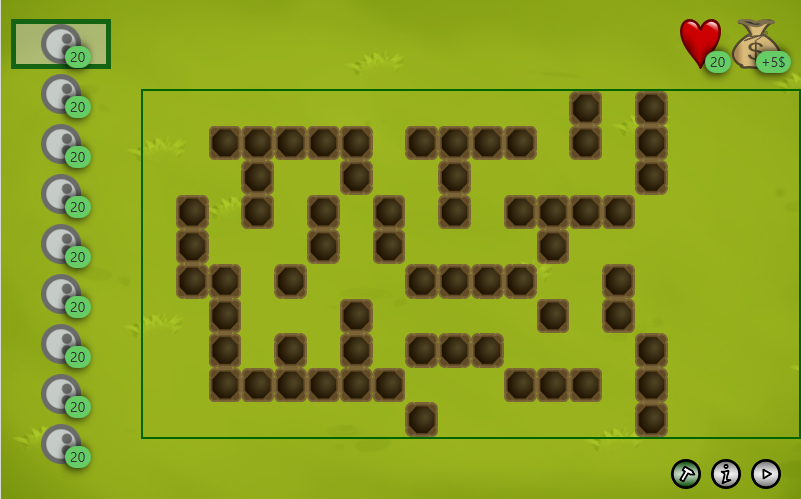
\includegraphics[width=8cm]{images/maze-runner-setup.png}
	\caption{Beispiel für ein Irrgarten-Setup bei dem eigenen Projekt.}
\end{figure}

\paragraph{State der Kreaturen} In den bisherigen Spielvarianten benötigten die Kreaturen keine eigene Repräsentation des Spielfeldes. Dagegen müssen die Creeps sich nun individuell auf Grundlage ihres bisherigen Wissens über die Spielwelt bewegen. Ein wichtiges Spielelement ist daher die Klasse \class{VisitedMap}, mit der jede Kreatur in einem zweidimensionalen Enum-Array dieses Wissen speichert. Andererseits sollen die Kreaturen auch über eine gewisse Intelligenz verfügen und nicht alle in die selbe Sackgasse laufen. Das gelingt durch simulierte Besprechungen zwischen den Kreaturen. Die Karten müssen also effizient synchronisierbar sein (siehe \ref{par:visitedmap}).

\paragraph{Wegfindung} Die effiziente Wegfindung ist ebenfalls schwieriger: Während bei normalen TD-Spielen gar keine Berechnung notwendig ist und bei Mazing TD ein A*-Algorithmus effizient den kürzesten Weg von allen Kartenpunkten zum Ziel berechnen kann, muss der Algorithmus hier noch weiter abgewandelt werden, da die Creeps ihr Ziel nicht kennen. Es muss daher für jeden Creep ein eigenes Ziel ausgewählt werden, was zum Beispiel durch Breitensuchen umgesetzt werden kann.

\paragraph{Variationsmöglichkeiten} Dadurch, dass die Kreaturen ihre eigene Wegfindung haben und Absprachen treffen, ergeben sich neue Möglichkeiten der Variation der Creeps. Beispielsweise wurden Figuren implementiert, die sich nur zufällig bewegen, andere versuchen jedes Feld der Spielwelt zu besuchen. Weitere Möglichkeiten wären Kreaturen, die tatsächlich sehen können und damit z.B. größere Flächen direkt durchqueren, oder Kreaturen die andere dirigieren. Auch neue Turmarten, die auf diese Wegfindung Einfluss haben, sind möglich. Als Beispiel wurde dafür ein Amnesie-Turm programmiert, der bei abgeschossenen Creeps bewirkt, dass sie sich eine Zeit lang zufällig bewegen.

\paragraph{Labyrinthänderungen} Die für das Genre typischen Echtzeit-Änderungen des Labyrinths sind in der Variante schwieriger an Kreaturen zu kommunizieren. Da die Creeps den Zustand ihrer erkundeten Spielwelt speichern, sind Änderungen in bereits erkundeten Bereichen problematisch. Es gibt mehrere Möglichkeiten damit umzugehen, die in der Entwicklung abgewogen und mit User-Testings betrachtet wurden:
\begin{itemize}
	\item Kreaturen erhalten kein Update über die Spielwelt. Bei dieser Lösung musste ein Verhalten implementiert werden, falls Creeps denken es gäbe keinen Ausweg. Typischerweise greifen eingesperrte Figuren die Türme an oder rennen darüber, was in der eigenen Variante so implementiert wurde. Das User Feedback zeigte, dass das Verhalten der Creeps insbesondere wegen der Kommunikation nicht nachvollziehbar ist.
	\item Kreaturen erhalten ein Update, falls sie den Bereich bereits erkundet hatten. Dies führte in User-Testings zu Strategien gegen das Spielprinzip, bei denen zwei Türme auf verschiedenen Seiten der Karte immer abwechselnd neu gebaut und später wieder abgerissen wurden, sodass die Kreaturen immer von einem Ende zum anderen laufen mussten.
	\item Türme können gar nicht abgerissen werden, oder nur, wenn kein lebender Creep diesen erkundet hat. Dies schränkt die Möglichkeiten der Spieler zwar ein, ist aber besser verständlich und bleibt dem Spielprinzip treu.
\end{itemize}
% subsection neuer_ansatz_im_eigenen_projekt (end)

\subsection{Reflexion der Projektdefinition} % (fold)
\label{sub:reflexion_der_projektdefinition}

Neben der oben ausführlich beschriebenen Projektidee formulierte die Projektdefinition bereits Details zur Umsetzung des fertigen Spiels aus User-Sicht und einige Mindestanforderungen sowie mögliche Erweiterungen. Im Folgenden soll diese Beschreibung noch einmal wiedergegeben werden, da sie ähnlich einem Lastenheft den Leitfaden für das Projekt bot.

\begin{quotation}
Die Spielansicht zeigt die Leben und das Geld des Spielers, eine Zeitlinie der nächsten Gegnergruppen,
sowie die Labyrinth-Ebene. In Letzterer kann der Spieler Mauern bauen und dann diese mit Türmen
aufrüsten. Es stehen verschiedene Türme zur Verfügung, die zudem während des Spiels durch
Upgrades verbessert werden können.
\end{quotation}
Diese Anforderung wurde exakt wie gefordert umgesetzt
\begin{quotation}
In mehreren Wellen werden entsprechend der Zeitlinie Gegner generiert, die mit unterschiedlichen
Strategien versuchen, den Ausgang des Labyrinths zu erreichen. Sie kommunizieren untereinander,
vermeiden also z.B. Sackgassen, die andere bereits erkundigt haben. Die Einheiten ändern somit
während dem Spiel dynamisch ihre Wegfindung.
\end{quotation}
Auch diese Anforderung ist umgesetzt worden und wird in den nächsten Kapiteln noch genauer beschrieben.

\begin{quotation}
Mindestanforderungen:
\begin{enumerate}
	\item Desktop-Anwendung \textcolor{dkgreen}{(erfüllt)}
	\item Grundfunktionalitäten eines Mazing-TD-Spiels (Leben, Geld, Mazing-Funktionalitäten, Pfadsuche
	der Computergegner) \textcolor{dkgreen}{(erfüllt)}
	\item Verschiedene Türme mit mehreren Upgradestufen \textcolor{dkgreen}{(erfüllt)}
	\item Verschiedene Gegnerarten \textcolor{dkgreen}{(erfüllt)}
	\item Kommunikation der Gegner untereinander bei Sackgassen \textcolor{dkgreen}{(erfüllt)}
	\item Rudimentäre Grafikgestaltung in JavaFX (Top Down Perspektive, einfaches Design) \textcolor{dkgreen}{(übertroffen)}
	\end{enumerate}
\end{quotation}
Neben den Mindestanforderungen, die ein spielbares und interessantes Spiel beschrieben, wurden noch einige mögliche Erweiterungen beschrieben, die nur zum Teil umgesetzt wurden. Dafür wurden bei der Entwicklung auf andere Sachen größeren Wert gelegt. 
\begin{quotation}
Erweiterungen
\begin{enumerate}
	\item Kampagnenmodus (Steigender Schwierigkeitsgrad, Story) \textcolor{dkred}{(nicht umgesetzt)}
	\item Tutorial für Spielsteuerung \textcolor{dkred}{(nicht umgesetzt)}
	\item Mehrere Karten (Andere Szenarie, mehrere Zugänge, ...) \textcolor{dkred}{(nicht umgesetzt)}
	\item Kompliziertere Strategien der Gegner (z.B. Auf Mauern klettern und andere Einheiten dirigieren) \textcolor{dkgreen}{(z.T. umgesetzt)}
	\item Strategiesteuerung für Türme (Angreifen des schwächsten/stärksten/nächsten/... Gegners) \textcolor{dkgreen}{(z.T. umgesetzt)}
	\item Anspruchsvollere Grafik (z.B. isometrische Perspektive) \textcolor{dkred}{(nicht umgesetzt)}
	\item Android-Anwendung \textcolor{dkgreen}{(erfüllt)}
	\item Mehrspielermodus (Große Karte, in der jeder Spieler einen Teil ausbaut) \textcolor{dkred}{(nicht umgesetzt)}
\end{enumerate}
\end{quotation}
Die Android-Anwendung wurde auf Kompatibilität bis Android 4.2.2 (Jelly Bean) getestet. Dafür waren einige Laufzeitoptimierungen notwendig, die systematisch gemessen und implementiert wurde, wie in den folgenden Kapiteln auch beschrieben wird. Neben diesem Feature wurde in das Projekt eine (De-) Serialisierung mit JSON eingebaut, sodass das aktuelle Spiel abgespeichert und neu geladen werden kann. Ein weiteres nicht genanntes Element bei der Entwicklung, das nicht in der Projektdefinition erwähnt war, ist das ausführliche UnitTesting, das in Kapitel~\ref{sub:testgetriebene_entwicklung} genauer beschrieben wird. 
% subsection reflexion_der_projektdefinition (end)
% section projektidee (end)